% ****** Start of file apssamp.tex ******
%
%   This file is part of the APS files in the REVTeX 4.1 distribution.
%   Version 4.1r of REVTeX, August 2010
%
%   Copyright (c) 2009, 2010 The American Physical Society.
%
%   See the REVTeX 4 README file for restrictions and more information.
%
% TeX'ing this file requires that you have AMS-LaTeX 2.0 installed
% as well as the rest of the prerequisites for REVTeX 4.1
%
% See the REVTeX 4 README file
% It also requires running BibTeX. The commands are as follows:
%
%  1)  latex apssamp.tex
%  2)  bibtex apssamp
%  3)  latex apssamp.tex
%  4)  latex apssamp.tex
%
\documentclass[%
 reprint,
%superscriptaddress,
%groupedaddress,
%unsortedaddress,
%runinaddress,
%frontmatterverbose, 
%preprint,
%showpacs,preprintnumbers,
%nofootinbib,
%nobibnotes,
%bibnotes,
 amsmath,amssymb,
 aps,
%pra,
%prb,
%rmp,
%prstab,
%prstper,
%floatfix,
]{revtex4-1}

\usepackage{graphicx}% Include figure files
\usepackage[utf8]{inputenc}
\usepackage{dcolumn}% Align table columns on decimal point
\usepackage{bm}% bold math
%\usepackage{hyperref}% add hypertext capabilities
%\usepackage[mathlines]{lineno}% Enable numbering of text and display math
%\linenumbers\relax % Commence numbering lines

%\usepackage[showframe,%Uncomment any one of the following lines to test 
%%scale=0.7, marginratio={1:1, 2:3}, ignoreall,% default settings
%%text={7in,10in},centering,
%%margin=1.5in,
%%total={6.5in,8.75in}, top=1.2in, left=0.9in, includefoot,
%%height=10in,a5paper,hmargin={3cm,0.8in},
%]{geometry}

\begin{document}

\preprint{APS/123-QED}

\title{Microondas}% Force line breaks with \\
\thanks{}%

\author{Jesus Prada}
 \email{jd.prada1760@uniandes.edu.co}
 \altaffiliation[Also at ]{Departamento de Física, Universidad de los Andes}%Lines break automatically or can be forced with \\
\author{Sergio Iv\'an Rey}%
 \email{si.rey1826@uniandes.edu.co}
\affiliation{%
 Departamento de Física, Universidad de los Andes
}%

\date{10/09/2015}% It is always \today, today,
             %  but any date may be explicitly specified

\begin{abstract}
Durante este laboratorio se pretendía estudiar los fenómenos ondulatorios de las microondas en distintas configuraciones. En primer lugar se verificó el ángulo de máxima reflexión de las microondas al hacerlas incidir sobre una película metálica. Se comprobó que el ángulo de mayor reflexión es el mismo ángulo que el ángulo incidente con una precisión de $\pm2^o$. Asimismo, durante varias prácticas se determinó experimentalmente la longitud de onda de las microondas. Esto se llevó a cabo usando, en primer lugar un montaje para simular ondas estacionarias con el receptor actuando como reflector parcial. En segunda instancia se midió la longitud de onda mirando el patrón de interferencia de una doble rendija. De la misma manera, se determinó esta longitud de onda usando los interferómetros de Fabry-Perot, Michelson y el espejo de Lloyd. Para todos los casos, se encontró una longitud de onda dentro de los límites esperados obteniendo así un valor con error mínimo dado por $\lambda = 2.86cm$ ($0.1\%$) y un error máximo dado por $\lambda= 2.22cm$ ($22\%$). Se midieron asimismo los fenómenos de polarización, haciendo uso de las cabezas movibles que disponía el equipo de microondas, en donde se encontró como era esperado, la relación de intensidad proporcional a la componente que se dejaba pasar. Similarmente, haciendo uso de partículas pequeñas de estireno ubicadas dentro de un prisma se comprobó el fenómeno de refracción y se comprobó la Ley de Snell, como también pudo encontrarse, con un valor del índice de refracción de $n = 1.41$ ($11\%$ de error) el cual es muy cercano al nominal. Finalmente, haciendo uso del estireno, se diseñó una manga llena de estas partículas que serviría como fibra óptica con la cual se comprobó que la onda se transmitía sin pérdida de energía por este elemento. \\
\end{abstract}


\keywords{Microondas, refracción, reflexión, interferencia, fibra óptica, espejo de Lloyd, interferómetro de Michelson, interómetro de Fabry-Perot, ondas estacionarias}%Use showkeys class option if keyword
                              %display desired
\maketitle

%\tableofcontents

\section{\label{sec:level1}Introducci\'on}

La teoría electromagnética clásica es una de las teorías más exitosas y consistentes. Con esta teoría, aplicando las adecuadas condiciones de frontera y suposiciones sobre los materiales y el espacio, se puede deducir la cuantificación de la forma en como se propaga la luz en diferentes medios y en interfaces de distintos medios. De esta manera, prácticamente partiendo de las ecuaciones de Maxwell, se pueden deducir principios fundamentales ópticos como la ley del plano de incidencia, la ley de reflexión, y la ley de refracción. Otros fenómenos tambien son consecuencia de esta teoría, como la existencia del ángulo de Brewster, la reflexión interna total, entre otros.\\

Si se aplican las ecuaciones del electromagnetismo en la materia, sobre una interfaz de dos medios distintos, se encontrará que las condiciones de frontera para el campo eléctrico $E$ y el campo magnético $B$, con respecto a la superficie de la interfaz estarán dadas por: \cite{Griffiths}\\

\begin{align*}
E_1^{\parallel} = E_2^{\parallel}\\
\epsilon_1E_1^{\perp} = \epsilon_2E_2^{\perp}\\
\frac{1}{\mu_1}B_1^{\parallel} = \frac{1}{\mu_2}B_2^{\parallel}\\
B_1^{\perp} = B_2^{\perp}\\
\end{align*}

Con la aplicación de estas condiciones sobre una onda incidente con ángulo de incidencia $\theta_I$ monocromática, se pueden obtener las leyes de reflexión y refracción:\cite{Griffiths}\\


\begin{equation}
	\theta_I = \theta_R
\label{eq:reflexion}
\end{equation}

\begin{equation}
	n_1\sin{\theta_I} = n_2sin{\theta_T}
\label{eq:refraccion}
\end{equation}

Donde $\theta_R, \theta_T$ hacen referencia a los ángulos de reflexión y refracción respectivamente, los cuales, al igual que el ángulo de incidencia, están definidos con respecto a la normal de la superficie de incidencia, por lo que solo pueden tomar valores en $[0,\frac{\pi}{2})$. Por otra parte, el índice de refracción $n$ se define como la razón entre la velocidad de la luz y la velocidad en el medio actual, y está relacionado con la densidad óptica del medio:\\

\begin{equation}
	n = \frac{c}{v} = \sqrt{\frac{\epsilon\mu}{\epsilon_0\mu_0}}
\label{eq:indice}
\end{equation}

Cabe resaltar que la ley del plano de incidencia, la cual dice que el rayo incidente, el reflejado y e transmitido se encuentran en un mismo plano que es perpendicular a la interfaz, es la que nos permite caracterizar completamente las direcciones del fenómeno de refracción y reflexión solo con los 3 ángulos mencionados.\\

De la ley de refracción cabe resaltar que si el medio de incidencia es más denso ópticamente que el medio de transmisión, existirá un ángulo de incidencia en el intervalo $[0,\frac{\pi}{2})$, tal que el ángulo de refracción tenga que ser exactamente $\frac{\pi}{2}$ para poder satisfacer la ley de Snell. Esta relación se expone en la ecuación \ref{eq:rit}. Con un posterior análisis sobre los coeficientes de transmisión y reflexión, que indican qué tanta luz se refleja y qué tanta luz se transmite, se puede concluir que para ángulos menores a este ángulo crítico, toda la luz es reflejada, y nada se transmite al otro medio. En estos casos, el ángulo de transmisión tendría que ser mayor a $\frac{\pi}{2}$ o menor a $0$, lo cual no cumple lo asumido por la ley del plano de incidencia. Este es el principio sobre el cual se basa el funcionamiento de la fibra óptica. Aquí, la fibra es tan delgada que el ángulo de incidencia siempre es menor que el ángulo crítico, por lo que siempre se da la reflexión interna total y no se pierde luz por transmisión.\\

\begin{equation}
	\sin{{\theta_I}_{crit}} = \frac{n2}{n1}\sin{\frac{\pi}{2}} < 1
\label{eq:rit}
\end{equation}

Ahora, para un conductor perfecto el campo dentro del conductor es nulo \cite{Griffiths}, dado que cualquier campo que se intente aplicar, moverá las cargas en la superficie del conductor de tal manera que lo anule. En este sentido, si se tiene una rejilla de un material conductor, se puede puede dejar pasar campo eléctrico solo en la dirección de la rejilla, dado que la componente del campo que no sea paralela, encontrará el conductor y se anulará. En este sentido, con una rejilla metálica se puede polarizar una onda electromagnética.\\

Si se se tiene luz polarizada incidente a un polarizador con un desfase en la dirección de polarización dado por $\theta_1$ respecto a la luz incidente, teniendo en cuenta que solo puede pasar la componente de campo eléctrico paralela al polarizador, la intensidad de la luz recibida estará dada por:\\

\begin{equation}
I = \frac{1}{2}\epsilon_0{E^{\parallel}}^2 = \frac{1}{2}\epsilon_0{E_0}^2{\cos^2{\theta_1}} \propto \cos^2{\theta_1}
\label{eq:polarizador}
\end{equation}

Si se pone otro polarizador en medio de estos dos, con desfase $\theta_2$ con respecto a la luz incidente, la intensidad estará dada al aplicar \ref{eq:polarizador} dos veces, teniendo en cuenta que el desfase entre los dos polarizadores es $\theta_1-\theta_2$:\\

\begin{equation}
I = \frac{1}{2}\epsilon_0{E_0}^2{\cos^2{\theta_2}}\cos^2{ \left( \theta_1-\theta_2 \right) } \propto \cos^2{ \theta_1}\cos^2{ \left( \theta_1-\theta_2 \right) }
\label{eq:polarizador2}
\end{equation}

Nótese que si la luz incidente es perpendicular al polarizador, si solo tenemos en cuenta un polarizador, $\theta_1 = \frac{\pi}{2}$ entonces la onda transmitida tendrá intensidad nula. sin embargo, si ponemos otro polarizador en medio, tendremos de forma general $\theta_1 - \theta_2 \neq \frac{\pi}{2}$ por lo que la onda transmitida no necesariamente tendrá intensidad nula.\\

Otro experimento que es sencillo de cuantificar con la teoría electromagnética es el experimento de la doble rendija. Si se hace incidir luz monocromática coherente sobre una placa conductora (no deja pasar luz) con una rendija doble con una separación $d$, se observará un patrón de difracción. Este patrón ondulatorio se debe al principio de superposición del campo electromagnético, el cual dice que el campo electromagnético en un punto debido a dos fuentes es la suma de los campos producidos por cada fuente por separado en dicho punto \cite{Griffiths}. Debido a esto, si consideramos ondas, la suma de ambos campos es dependiente de la fase. Si se hace un análisis de los caminos que toman las ondas que pasan por cada una de las rendijas se llegará a la conclusión de que la interferencia destructiva se da cuando:\\


\begin{equation}
d\sin{\theta} = n\lambda
\label{eq:interferencia}
\end{equation}

Donde $\theta$ se refiere al ángulo respecto al centro de la rejilla de difracción donde se toma la medida de intensidad de la luz.\\

Con el experimento de la doble rendija se puede introducir al campo de la interferometría, donde se busca medir distancias del orden de la longitud de onda con la que se trabaja, al mirar la patrones de interferencia o simplemente la distancia entre los máximos o mínimos que ocasiona la superposición de dos haces de luz que han tomado caminos diferentes. El principio de interferencia por diferencia de fases de haces de luz es el principio detrás de experimentos importantes actuales como los detectores de ondas gravitacionales, y de experimentos que hicieron historia como el de Michelson-Morley.\\

Una de las formas de hacer interferometría con ondas esféricas es el espejo de Lloyd. En dicho montaje, mostrado en la figura \ref{fig:espejo} se tiene un material conductor paralelo a la dirección emisor-receptor, situado a mitad de camino entre estos dos instrumentos, cuya distancia perpendicular se puede variar para provocar interferencia entre la onda que se refleja en el conductor y la onda que toma el camino emisor-receptor. Un análisis sencillo de la diferencia de caminos, asumiendo que la onda se propaga esféricamente, nos dice que hay interferencia constructiva cuando se tiene:\\

\begin{equation}
D-2{\left(d^2 + {\left(\frac{D}{2}\right)}^2\right)}^\frac{1}{2} = n\lambda
\label{eq:Lloyd}
\end{equation}

Donde $D$ es la distancia del receptor al emisor, $d$ es la distancia del espejo al centro de la trayectoria, $\lambda$ es la longitud de onda de la luz incidente, y $n$ es un entero.\\

De este experimento de interferometría se puede notar claramente que la condición de interferencia no es lineal, y que además, al alejar el espejo, se disminuye la intensidad de la onda que se refleja (asumiendo que se propaga esféricamente), lo cual altera un poco la condición de interferencia.\\

Un experimento de interferometría que no es afectado por estos factores de no linealidad y de variación de la intensidad, es el interferómetro de Michelson y el de Fabry-Perot. Estos interferómetros trabajan bajo el mismo principio y lo único que los diferencia es el ordenamiento espacial de los elementos. El experimento de Michelson es mostrado en la figura \ref{fig:intmichelson} y consiste en superponer dos haces de luz que han tomado distintos caminos con la ayuda de un material semi-transparente. El de Fabry-Perot es análogo (figura \ref{fig:fabryperot}, sin embargo, los materiales semi-transparentes no están dispuestos a $45^o$ sino en medio del receptor y el transmisor.  En este caso, la relación de interferencia para máximos es simple de deducir y simple en general:\\

\begin{equation}
d = n\frac{\lambda}{2}
\label{eq:Michelson}
\end{equation}

Donde $d$ es la distancia a la que se corre el receptor o el emisor , entre dos máximos o mínimos. \\

De esta manera, muchos otros fenómenos ópticos pueden ser caracterizados con la teoría electromagnética clásica, sin embargo, no es objetivo de este informe describirlos todos .\\ 


\section{\label{sec:level1}Montaje experimental}

Durante la práctica se utilizó el equipo de microondas de PASCO modelo WA-9314B y se siguieron cuidadosamente las instrucciones detalladas de la guía del usuario \cite{guia}.\\

\subsection{\label{sec:level2}Reflexión de Microondas}
Para esta manipulación, se configuró el montaje que se muestra en la figura \ref{fig:reflexion} .\\

\begin{figure}[h!]
\centering
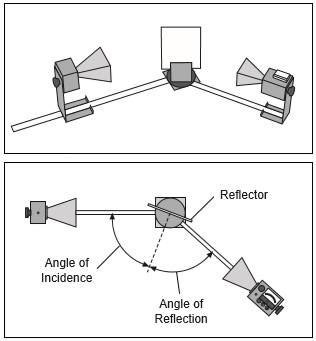
\includegraphics[width=0.7\linewidth]{Pictures/reflexion}
\caption{Montaje experimental - Refelxión de Microondas}
\label{fig:reflexion}
\end{figure}

A continuación, dejando el emisor de ondas fijo, a un ángulo de $45^o$ con respecto a la normal del reflector, se procedió a mirar para qué ángulo el receptor mostraba una señal máxima. Se encontró que $45^o$ era el máxmimo de la señal. Esto se hizo para verificar el montaje. \\

Acto seguido, la intensidad del receptor se ajustó en 30X para asegurarse de detectar las más pequeñas variaciones, y se procedió a mover el ángulo incidente desde $20^o$ a $90^o$. El receptor se movió angularmente hasta detectar un máximo. De allí se pudo inferir la relación entre el ángulo incidente y el ángulo reflejado.  \\

Debe anotarse que dado que las ondas son esféricas, hay una medición extra dado que la onda recibida por detector no es sólamente la reflejada sino también se suma una porción directamente proveniente del emisor.\\

\subsection{\label{sec:level2}Refracción a través de un prisma}

Para esta manipulación se configuró el montaje mostrado en la figura \ref{fig:refraccion}. El compartimiento triangular del centro actuaba como prisma. \\

\begin{figure}[h!]
\centering
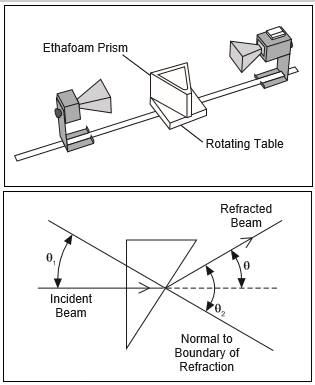
\includegraphics[width=0.7\linewidth]{Pictures/refraccion}
\caption{Montaje Experimental - Refracción por prisma}
\label{fig:refraccion}
\end{figure}
 
En primer lugar, se procedió a determinar la influencia de este material en la señal del receptor y una vez demostrado que la diferencia era prácticamente nula, se rellenó el interior del prisma con partículas de estireno.\\ 

Con el emisor de ondas fijo, se procedió a mover el detector hasta detectar un máximo en la señal.  Se denota, $ \theta $ el ángulo que marca directamente el detector con el goniómetro. \\

Una vez hallado este ángulo, con el diagrama de la figura \ref{fig:refraccion} se pueden determinar los ángulos incidente y refractado y así hallar el coeficiente de refracción del estireno por medio de la Ley de Snell. \\

En este caso, el medio incidente es el estireno.\\
 
\subsection{\label{sec:level2}Polarización}

Este experimento tuvo dos partes. En primer lugar, el montaje consistía en el que se muestra en la figura \ref{fig:polarizador1} con la excepción de que no había una rejilla de polarización en el medio. Con esto, receptor y emisor frente a frente se procedió a mover el cuerno del detector de ondas dejando el receptor fijo. De esta manera, las ondas producidas impactarían el detector con diferentes ángulos de polarización. \\ 

\begin{figure}[h!]
\centering
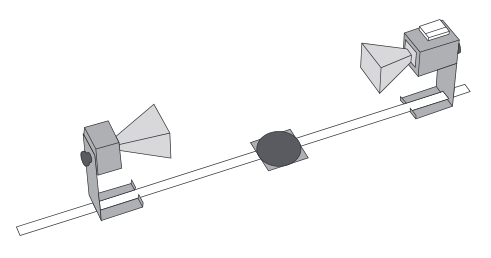
\includegraphics[width=0.7\linewidth]{Pictures/polarizador1}
\caption{Montaje Experimental - Polarización}
\label{fig:polarizador1}
\end{figure}

Se midieron así, en aumentos de $5^o$ las señales recibidas para un rango de ángulos de polarización entre $0^o$ y $90^o$. \\

En la segunda parte se prepararon el emisor y el receptor con direcciones paralelas de polarización, se incluyó la rejilla de polarización imitando el montaje en la figura \ref{fig:polarizacion}, y ésta se ubicó en ángulo de $0^o$,$22.5^o$,$45^o$, $67.5^o$ y $90^o$ con respecto al ángulo del emisor. Luego se  se repitieron las medidas para $0^o$, $45^o$ y $90^o$, esta vez configurando el emisor y el receptor en direcciones perpendiculares de polarización.\\ 

\begin{figure}[h!]
\centering
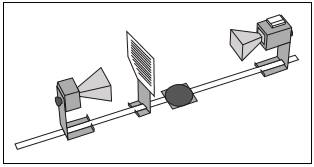
\includegraphics[width=0.7\linewidth]{Pictures/polarizacion}
\caption{Montaje Experimental - Polarización 2}
\label{fig:polarizacion}
\end{figure}

\subsection{\label{sec:level2}Determinación de $ \lambda $}
\textit{Interferencia de doble rendija} \\

\begin{figure}[h!]
\centering
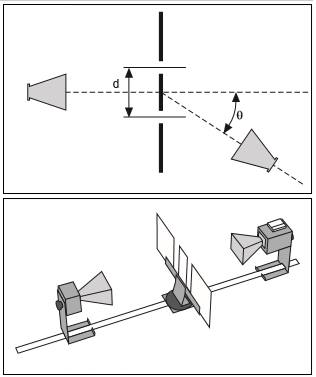
\includegraphics[width=0.7\linewidth]{Pictures/Interferencia}
\caption{Montaje Experimental - Interferencia a Doble Rendija}
\label{fig:Interferencia}
\end{figure}

En este experimento se armó el montaje mostrado en la figura \ref{fig:Interferencia}. Dejando el emisor de ondas fijo, se movió el detector a través del ángulo $ \theta $ mostrado en la figura. Para un barrido de este ángulo entre $0^o$ y $85^o$ en aumentos de $5^o$, se anotó el valor de la intensidad detectada por el receptor. \\

Se repitieron las medidas cambiando la distancia de separación entre rendijas.\\ 

\textit{Ondas estacionarias} \\

Para medir ondas estacionarias se utilizó como reflector el detector mismo. Se ubicaron frente a frente ambos equipos como se muestra en la figura \ref{fig:estacionarias}. \\

\begin{figure}[h!]
\centering
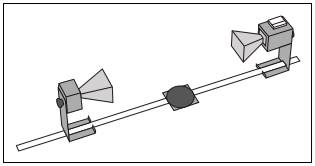
\includegraphics[width=0.7\linewidth]{Pictures/estacionarias}
\caption{Montaje Experimental - Ondas estacionarias}
\label{fig:estacionarias}
\end{figure}

A continuación, se ubicó el detector en donde éste mostrara la lectura de un máximo, y acto seguido se procedió a deslizar el detector hacia atrás. En dos manipulaciones diferentes, se contaron 20 y 30 máximos respectivamente y se procedió a determinar $ \lambda $ con la fórmula para los máximos de una onda estacionaria, la cual es la misma condición presentada en la ecuación \ref{eq:Michelson}. \\ 

\textit{Espejo de Lloyd} \\

Para determinar $ \lambda $ se utilizó también el montaje del espejo de Lloyd mostrado en la figura \ref{fig:espejo}. En este caso el receptor mostrará una señal máxima cuando ambos caminos recorridos por la onda emitida estén en fase. \\

\begin{figure}[h!]
\centering
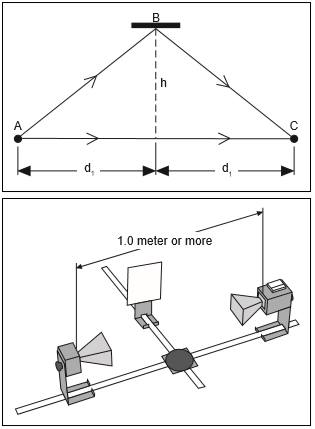
\includegraphics[width=0.7\linewidth]{Pictures/espejo}
\caption{Montaje Experimental - Espejo de Lloyd}
\label{fig:espejo}
\end{figure}

Para medir este fenómeno se dejan reflector y emisor fijos, separados a una distancia idéntica desde el centro del sistema y se desplaza el reflector hacia atrás. \\

En primer lugar, debe ubicarse el reflector en el primer mínimo que sea posible detectar y acto seguido desplazarlo hacia atrás hasta encontrar cuando menos 10 mínimos de intensidad. De esta forma, la diferencia de caminos debe cumplir la ecuación \ref{eq:Lloyd} para producir interferencia constructiva\\

La medición se realizó dos veces para diferentes separaciones entre emisor y receptor.\\


\textit{Interferómetro de Fabry-Perot} \\

En este caso se recreó el interferómetro de Fabry-Perot, haciendo uso del montaje mostrado en la figura \ref{fig:fabryperot}. Durante esta manipulación se pretendía encontrar la longitud de onda así que se procedió de manera similar al experimento de ondas estacionarias y al espejo de Lloyd.\\


\begin{figure}[h!]
\centering
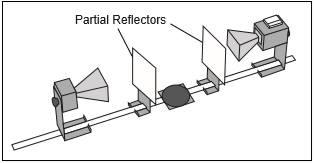
\includegraphics[width=0.7\linewidth]{Pictures/fabryperot}
\caption{Montaje Experimental - Interferómetro de Fabry-Perot}
\label{fig:fabryperot}
\end{figure}

Dejando el emisor fijo se ubicó el receptor en un mínimo. Acto seguido, se procedió a mover el mismo hacia atrás hasta haber pasado por n mínimos de intensidad. Así pues, con la fórmula \ref{eq:Michelson}, se determinó la longitud de onda. \\ 

\textit{Interferómetro de Michelson} \\

En este experimento se trató de recrear el experimento de Michelson-Morley con microondas, haciendo uso del montaje mostrado en la figura \ref{fig:intmichelson}. \\

\begin{figure}[h!]
\centering
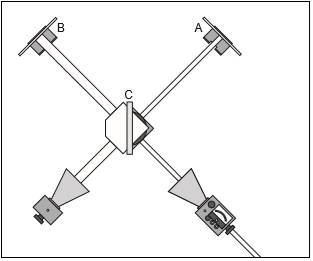
\includegraphics[width=0.7\linewidth]{Pictures/intmichelson}
\caption{Montaje Experimental - Interferómetro de Michelson}
\label{fig:intmichelson}
\end{figure}

Se ubicó el detector en el mínimo más cercano encontrado con respecto al centro del sistema y se procedió a deslizar el equipo hacia atrás contando mínimo diez mínimos de intensidad. Con una fórmula similar a las utilizadas anteriormente, se determinó $ \lambda $. \\

La fórmula utilizada es la misma que para el interferómetro de Fabry-Perot. \\


\subsection{\label{sec:level2}Fibra Óptica}

Para el experimento de fibra óptica se utilizaron nuevamente las partículas de estireno, sólo que en esta ocasión se configuró una suerte de fibra óptica al ponerlas de relleno en una bolsa larga de plástico. \\

El experimento es de énfasis cualitativo y consistió en estudiar cómo, por medio de la fibra óptica, el detector puede leer la intensidad de la onda incidente en diferentes configuraciones. \\

Dichas configuraciones consistían en mover el cuerno del emisor y el receptor cambiando el ángulo de polarización como también ver cómo cambiaba la señal al cambiar la curvatura de la fibra. \\ 

Se quería comprobar también que si uno de los extremos no se encontraba debidamente introducido en los cuernos de los equipos, la lectura sería cero. \\


\section{\label{sec:level1}Resultados y An\'alisis}

\subsection{\label{sec:level2}Reflexión de Microondas}

Al mover el ángulo de incidencia, la máxima señal recibida también cambiaba. Al final, se encontró, como se esperaba por la teoría electromagnética, que el ángulo de incidencia y el ángulo de reflexión son el mismo con un error de $2^o$ en promedio para cada medida. \\

Hay que anotar que para valores grandes, las mediciones se atrofiaban puesto que se estaba recibiendo, principalmente, la onda directamente en lugar de una proción reflejada. \\

\begin{table}[h!]
\centering
\begin{tabular}{|c|c|}
	\hline $ \theta_I (^o) $ & $ theta_R ( \pm 1^o  )$  \\ 
	\hline\hline
	20 &  21\\ 
	30 &  32\\ 
	40 &  41\\ 
	50 &  51\\ 
	60 &  59\\ 
	70 &  69\\ 
	80 &  78\\ 
	90 &  78\\ 
	[1ex] 
 \hline
 \end{tabular} 
  \caption{Ángulos de reflexión}
\label{table:incref} 
\end{table}

Los datos se encuentran consignados en la tabla \ref{table:incref}. \\

\subsection{\label{sec:level2}Refracción a través de un prisma} 

En primer lugar, para tomar en cuenta la refracción causada por el triángulo, se demostró que éste no hacía mayor cambio en la señal recibida. Así pues, se procedió a determinar el índice de refracción del estireno. \\

Para la máxima lectura, se tuvo $ \theta = 10 \pm 1^o $. Por la configuración misma del sistema, se tiene que en el diagrama de la figura \ref{fig:refraccion}, $ \theta_1 = \phi = 20\pm1^o $, siendo $ \phi $ el ángulo menor del triángulo que conforma el prisma. \\

Así, se tiene que $ \theta_2 = \theta_1 + \theta = 30\pm1^o $. Asumiendo el ínidce de refracción del aire como 1, se tiene con la ecuación \ref{eq:refraccion}:

\begin{equation}
\frac{n_1}{n_2} = \frac{\sin{\theta_2}}{\sin{\theta_1}}= 1.462\pm0.08
\end{equation}

De esta manera, puesto que $ n_2 = 1 $, encontramos que el índice de refracción del estireno es precisamente $1.4162\pm0.08$, donde el error absoluto fue calculado con propagación de error sobre la fórmula usada. \\

El valor teórico está en 1.5916, lo cual demuestra un error absoluto del $11\%$, lo cual no está mal al considerar las distintas fuentes de error. Estas fuentes de error confluyen en la aguja del receptor, la cual es muy sensible y puede ser perturbada por factores ambientales electromagnéticos o por factores físicos como el movimiento de la mesa, el cual no era nada suave dada la fricción con los instrumentos. A veces, incluso, el receptor se apagaba debido a su batería baja. Esto fué corregido solo cuando fue muy evidente.\\


\subsection{\label{sec:level2}Polarización}
En este experimento no necesitabamos calcular ningún valor experimental, sino verificar que se cumplía la  relación de intensidad para el paso de luz a través de uno o dos polarizadores. Dicha relación puede ser recordada con las ecuaciones \ref{eq:polarizador} y \ref{eq:polarizador2}.\\

En primera instancia se midió la relación de polarización sin polarizadores. Esto se pudo hacer dado que el emisor emitía luz polarizada, y el receptor estaba polarizado, es decir, solo detectaba la componente de la luz que llegaba que era paralela a su dirección de polarización. En este caso, se pudo cubrir un rango amplio con bastantes mediciones, lo cual está consignado en la tabla \ref{table:polarizador1}.\\

\begin{table}[h!]
\centering
\begin{tabular}{|c|c|}
	\hline $ \theta (\pm 1^o) $ & $ I(\pm 0.2\cdot 10^{-1}mA  $)  \\ 
	\hline\hline
	0  &  0.0\\
	10 &  0.2\\
	20 &  1.0\\ 
	30 &  2.4\\ 
	40 &  4.4\\ 
	50 &  6.2\\ 
	60 &  7.2\\ 
	70 &  8.6\\ 
	80 &  9.2\\ 
	90 &  9.6\\ 
	100 &  9.2\\ 
	110 &  8.4\\ 
	120 &  7.4\\ 
	130 &  6.2\\ 
	140 &  4.2\\ 
	150 &  2.4\\ 
	160 &  0.8\\ 
	170 &  0.2\\ 
	180 &  0.0\\ 
	[1ex] 
 \hline
 \end{tabular} 
  \caption{Intensidad de polarización a diferentes ángulos.}
\label{table:polarizador1} 
\end{table}

Dado que no debemos cuantificar nada, lo único que resta hacer es una gráfica de los puntos comparada con la gráfica teórica de la relación de la ecuación \ref{eq:polarizador}. Cabe resaltar que la escala angular estaba desfasada un valor de $90^o$ y los datos se tomaron con esta escala. En otras palabras, en $0^o$, el receptor y el emisor tenían polarizaciones perpendiculares. Para graficar los datos con la relación es necesario tener en cuenta este desfase. Esta gráfica se puede apreciar en la figura \ref{fig:polarizador1}. \\


\begin{figure}[h!]
\centering
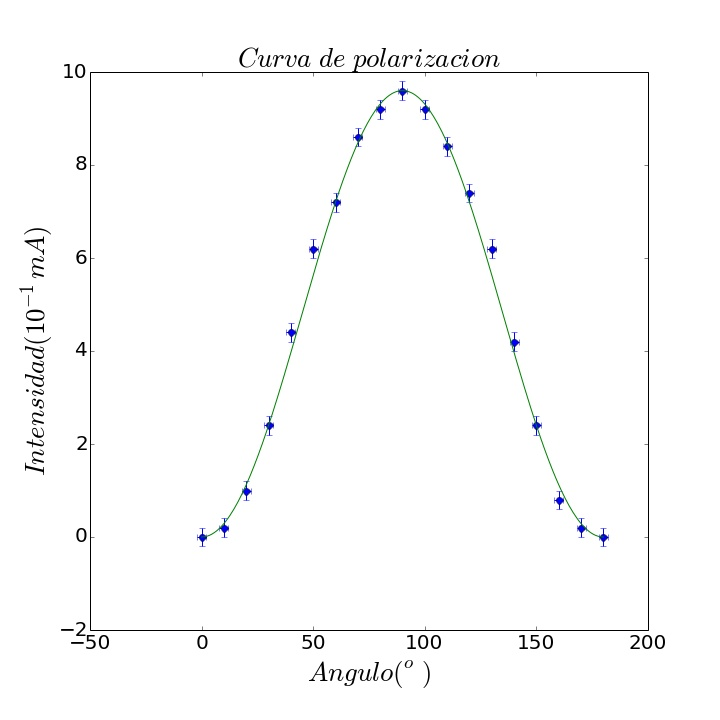
\includegraphics[width=0.8\linewidth]{polarizador1}
\caption{Intensidad contra ángulo de polarización}
\label{fig:polarizador1}
\end{figure}

En esta figura se puede apreciar la gran correlación de la relación de interferencia con los datos obtenidos. Eso se lo podemos atribuir a la simplicidad del montaje, que no contaba con otros elementos que provocaran fuentes de error además de los necesarios emisor y receptor.\\

En segunda instancia, medimos esta misma curva de intensidad contra ángulo de polarización preparando el emisor y receptor en direcciones de polarización paralela, esta vez, superponiendo un polarizador metálico en el medio al cual se variaba su dirección de polarización. En este caso, dada la polarización intrínseca del emisor y el receptor, esto equivale a un montaje con dos polarizadores, por lo que la ecuación que aplica aquí es la \ref{eq:polarizador2}. Debido a que tenemos al emisor y al receptor preparados en ángulos paralelos, para aplicar la ecuación, tendremos la condición $\theta_2 = 0$. Dicha ecuación tendrá entonces una dependencia de $\cos^4{(\theta_1)}$. Cabe resaltar que esta vez se cambió el ángulo del polarizador de metal manualmente sin tener una escala angular de referencia, por lo que los errores de ángulo pueden ser bastante grandes. Los datos obtenidos en este experimento se encuentran entonces en la tabla \ref{table:polarizador2} y la gráfica de los datos y su respectiva relación funcional se encuentran expuestas en la gráfica \ref{fig:polarizador2}. \\

\begin{table}[h!]
\centering
\begin{tabular}{|c|c|}
	\hline $ \theta (\pm 5^o) $ & $ I(\pm 0.2\cdot 10^{-1}mA  $)  \\ 
	\hline\hline
	0  &  7.8\\
	22.5 &  6.0\\ 
	45 &  2.2\\ 
	67.5 &  0.4\\ 
	90 &  0.0\\ 
	[1ex] 
 \hline
 \end{tabular} 
  \caption{Intensidad de polarización a diferentes ángulos.\\ Emisor-Receptor en orientación paralela}
\label{table:polarizador2} 
\end{table}

\begin{figure}[h!]
\centering
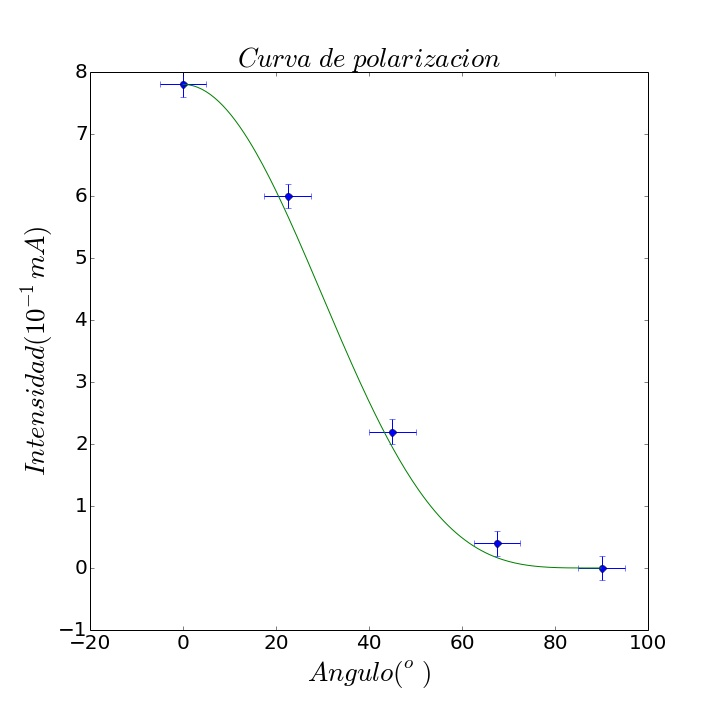
\includegraphics[width=0.8\linewidth]{polarizador2}
\caption{Intensidad contra ángulo de polarización \\ Emisor-Receptor en orientación paralela}
\label{fig:polarizador2}
\end{figure}

En esta gráfica se puede apreciar otra vez la buena dependencia predicha por la respectiva relación de intensidad dada por la respectiva ecucación. La curva entra en general en el rango dado por los errores, sin embargo, es preciso decir que dichos errores están siendo de todas maneras subestimados, especialmente el del la medición de intensidad, la cual variaba mucho con perturbaciones físicas de la mesa o ambientales electromagnéticas.\\

En última instancia, para el experimento de polarización, preparamos el emisor y el receptor en estados con dirección de polarización perpendicular. De la misma manera superpusimos un polarizador metálico al que variábamos su ángulo de polarización. En este caso, la ecuación que gobierna la curva de intensidad contra el ángulo de orientación de polaridad, es la misma ecuación \ref{eq:polarizador2}. Sin embargo, dada la perpendicularidad de las direcciones del emisor y el receptor, la condición aca es $\theta_2 = 90^o$. Así, la relación mencionada queda proporcional a $\left(\sin{(\theta_1)}\cos{(\theta_2)}\right)^2$. Los datos obtenidos se encuentran en la tabla \ref{table:polarizador3}.\\

\begin{table}[h!]
\centering
\begin{tabular}{|c|c|}
	\hline $ \theta (\pm 5^o) $ & $ I(\pm 0.2\cdot 10^{-1}mA  $)  \\ 
	\hline\hline
	0  &  0.0\\
	45 &  2.4\\ 
	90 &  0.0\\ 
	[1ex] 
 \hline
 \end{tabular} 
  \caption{Intensidad de polarización a diferentes ángulos.\\ Emisor-Receptor en orientación perpendicular}
\label{table:polarizador3} 7.
\end{table}

En este caso se tomaron únicamente 3 datos que verifican de una buena manera la relación intensidad contra los ángulos de polarización. En este caso podemos ver que cuando pusimos el polarizador metálico a $0^o$ y a $90^o$ no se detectó señal en el emisor. Esto se debe a que en un caso $\sin{(\theta_1) }= 0$ y en el otro caso $\cos{(\theta_1)} = 0$. Esto confirma indirectamente la ecuación \ref{eq:polarizador2}. En el caso de $45^o$, ninguno de los elementos se cancela, por lo cual obtuvimos un resultado no nulo que también confirma la ya mencionada ecuación.\\

\subsection{\label{sec:level2}Interferencia a Doble Rendija}
En este experimento cuantificamos el patrón de interferencia del experimento de doble rendija variando dos veces la distancia entre las rendijas. En primera instancia usamos una distancia de separación $d_1= 10.5cm$ para lo cual obtuvimos un buen patrón de interferencia. En segunda instancia, separamos las rejillas una distancia $d_2 = 7.4cm$, y debido a la relación en la ecuación \ref{eq:interferencia}, los mínimos de interferencia estaban más separados por lo que el patrón se veía más difuso.  Los datos obtenidos se encuentran en la tabla \ref{table:inter}.\\


\begin{table}[h!]
\centering
\begin{tabular}{|c|c|c|}
	\hline $ \theta (\pm 3^o) $ & $ I_1(\pm 0.2\cdot 10^{-1}mA  $) &$ I_2(\pm 0.2\cdot 10^{-1}mA)  $  \\ 
	\hline\hline
	0  &  10.0 & 10.0\\
	5  &  4.4 & 4.0\\
	10 &  0.1 & 0.8\\
	15 &  2.0 & 0.2\\
	20 &  3.0 & 1.0\\ 
	25 &  2.0 & 1.2\\ 
	30 &  0.2 & 0.2\\ 
	35 &  1.0 & 0.0\\ 
	40 &  0.4 & 0.0\\ 
	45 &  0.2 & 0.2\\ 
	50 &  0.4 & 0.4\\ 
	55 &  0.2 & 0.2\\ 
	60 &  0.2 & 0.0\\ 
	65 &  0.0 & 0.0\\ 
	70 &  0.0 & 0.0\\ 
	75 &  0.2 & 0.0\\ 
	80 &  0.0 & 0.0\\ 
	85 &  0.0 & 0.0\\ 
	[1ex] 
 \hline
 \end{tabular} 
  \caption{Patrón de interferencia para $d_1$ y $d_2$}
\label{table:inter} 
\end{table}

En este caso se escogieron $3^o$ como error absoluto en la medida del ángulo, porque experimentalmente, en este rango, el receptor arrojaba señales muy similares.\\

Una buena manera de proceder en este análisis de datos sería hacer un ajuste funcional de los datos teniendo en cuenta que estos deberían cumplir la ecuación de difracción de Fraunhofer superpuesta con la ecuación de intensidad para doble rendija, y luego mirar los mínimos de acuerdo al ajuste. Sin embargo, este ajuste no logró ser realizado con precisión. Una de las razones la falla del ajuste es que la ecuación para intensidad en términos del ángulo tiene una dependencia funcional de $\frac{\sin{(\alpha \theta)}}{\alpha\theta}$ lo cual tiene complicaciones numéricas alrededor de $\theta= 0$. Otra de las razones para la falla del ajuste, es que para poder aplicar la relación de interferencia, se necesita que los caminos de las ondas sean muy similares para que la diferencia de intensidades en el punto de interferencia sea despreciable. Esto se cumple cuando se mira el patrón de interferencia a una distancia $D$ mucho mayor que la separación de las rendijas $d$, lo cual no se cumplía para nuestro experimento. Por esto, se procedió a encontrar los mínimos del patrón de interferencia manualmente para mirar cómo cumplen la relación de interferencia dada por la ecuación \ref{eq:interferencia}.\\

Los datos pueden ser apreciados de manera más gráfica en las figuras \ref{fig:inter1} y \ref{fig:inter2}.\\

\begin{figure}[h!]
\centering
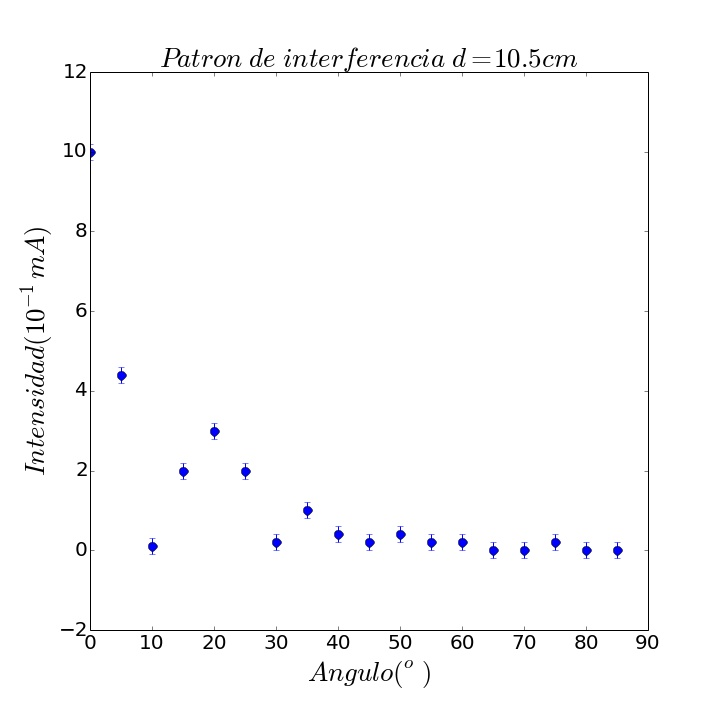
\includegraphics[width=1\linewidth]{inter1}
\caption{Patrón de interferencia para $d_1 = 10.5cm$}
\label{fig:inter1}
\end{figure}

\begin{figure}[h!]
\centering
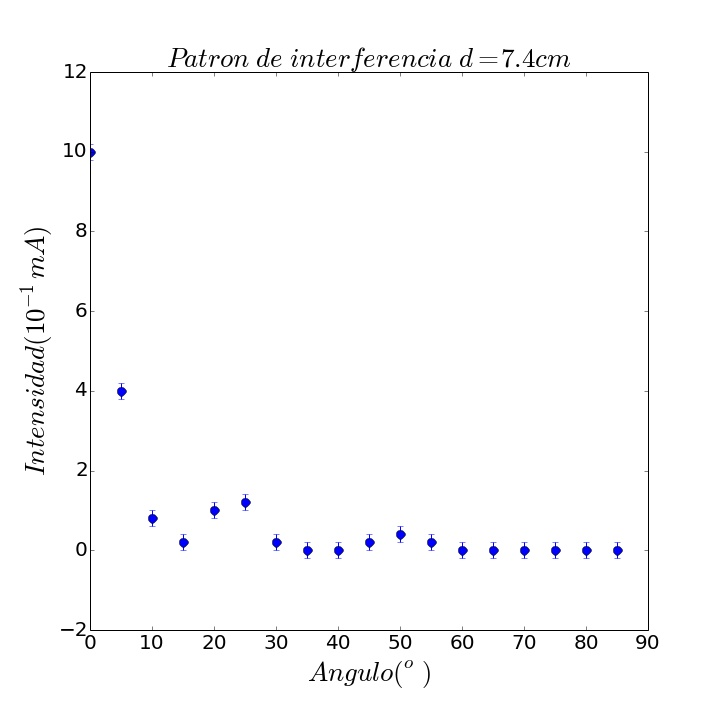
\includegraphics[width=1\linewidth]{inter2}
\caption{Patrón de interferencia para $d_2 = 7.4cm$}
\label{fig:inter2}
\end{figure}

De aquí se pueden deducir manualmente los primeros  tres mínimos de cada partrón, los cuales están dados por la tabla \ref{table:minimos}. Para los mínimos de orden mayor, el patrón de interferencia se vuelve muy ténue, y a falta de un ajuste, los mínimos ya no pueden ser determinados manualmente.\\


\begin{table}[h!]
\centering
\begin{tabular}{|c|c|c|}
	\hline $n $ & $ \theta_1 (\pm 3^o) $ & $ \theta_2 (\pm 3^o) $ \\ 
	\hline\hline
	1 & 10 & 15 \\
	2 & 30 & 35 \\
	3 & 45 & 60 \\
	[1ex] 
 \hline
 \end{tabular} 
  \caption{Mínimos de interferencia para $d_1$ y $d_2$}
\label{table:minimos} 
\end{table}

Si se toma el $\sin{\theta}$ para cada mínimo y se grafican los valores de la tabla anterior, se puede apreciar la relación lineal dada por la ecuación \ref{eq:interferencia}. Esta gráfica puede ser ajustada linealmente con la rutina de optimización de Scipy, en Python. Los respectivos ajustes pueden ser apreciados en  la gráfica \ref{fig:inter3}.\\

\begin{figure}[h!]
\centering
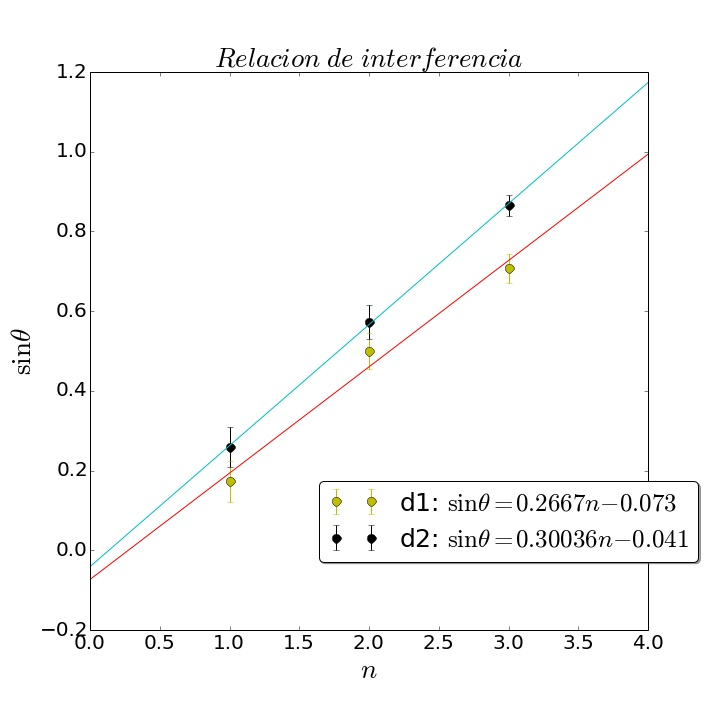
\includegraphics[width=0.8\linewidth]{inter3}
\caption{Relación de interferencia para $d_1$ y $d_2$}
\label{fig:inter3}
\end{figure}

De este ajuste lineal es importante notar que los valores de corte con el eje y son muy pequeños, como es esperado de una relación lineal como la ecuación \ref{eq:interferencia}. Además de esto, se puede obtener un estimado del error en la pendiente, dado por el ajuste. En este sentido, el valor de pendiente  en cada caso está dado por $m_1 = 0.2667 \pm 0.034$ y $m_2 = 0.300 \pm 0.006$. \\

Finalmente, para sacar el estimado de longitud de onda en cada caso solo es necesario multiplicar por las respectivas distancias $d_1$ y $d_2$. En este caso, teniendo en cuenta que el error asociado a cada medida de distancia es de $0.1cm$, haciendo la respectiva propagación de error, obtenemos las longitudes de onda dadas por $\lambda_1 = 2.79 \pm 0.36cm$ y $\lambda_2 = 2.22 \pm 0.05cm$.\\

De estos valores, es importante notar que respecto al valor teórico de $\lambda$, el primero cae en el rango de error y el segundo no. Esto se debe a la difusión del segundo patrón antes mencionado y al error humano introducido por la determinación manual de los mínimos de interferencia, lo cual era más dificil de determinar en dicho patrón. Por otra parte, los errores relativos al valor teórico están dado por $2.1\%$ y $22.1\%$ respectivamente.\\

\subsection{\label{sec:level2}Ondas estacionarias}
En este experimento tomamos el valor de longitud de onda de las microondas generadas por el emisor midiendo la distancia de separación de un número determinado de máximos de señal de onda estacionaria usando el mismo receptor como reflector parcial. Replicamos este experimento variando el número de máximos medidos, y los resultados, con sus respectivos errores, se encuentran en la tabla \ref{table:estacionaria}.\\

\begin{table}[h!]
\centering
 \begin{tabular}{|c|c|c|c|} 
 \hline
 $N Maximos$& $x_0(cm) \pm 0.1cm$ & $x_f(cm) \pm 0.1cm$ & $\lambda_{exp} (cm)$ \\ [0.5ex] 
 \hline\hline
 20 & 56 & 27.1 & 2.890 $\pm$ 0.01\\
 30 & 56 & 9.9 & 3.073 $\pm$ 0.006\\
[1ex] 
 \hline
 \end{tabular}
 \caption{Máximos de ondas estacionarias}
 \label{table:estacionaria}
\end{table}

Aquí, dado que la relación es lineal, y al igual que el experimento de Fabry-Perot y de Michelson, está dada por la ecuación \ref{eq:Michelson}, los errores tomados para los valores de la longitud de onda $\lambda$ fueron tomados con esta misma ecuación teniendo en cuenta únicamente el error aportado por el límite de resolución de la regla utilizada.\\

Los errores absolutos asociados a la medición son muy  pequeños, pero esto se debe a que no pudimos cuantificar la fuente más importante de error en este experimento, la cual provenía del receptor. En este caso determinar un máximo o un mínimo en la escala de intensidad analógica del receptor era muy difícil dado que este instrumento era muy sensible y tenía muchas fluctuaciones. Estas fluctuaciones se pueden deber a la contaminación electromagnética ambiental, o que a veces, nuestros mismos cuerpos podían actuar como reflectores y afectar la medición. Además, la mesa no era tan lisa para poder mover el espejo conductor de una manera suave que no perturbara la aguja de la medida.\\

El valor teórico de la longitud de onda emitida por estos instrumentos está dado por $\lambda_{teo} = 2.857 cm$, por lo que podemos deducir que el error relativo a la medida de $\lambda$ en cada caso, está dado por $0.5\%$ y $7.7\%$. De estos resultados es interesante notar que la medida que debía dar menor error relativo (la de 30 máximos) debido al poco error absoluto, dio mayor error. Esto se debe principalmente a que a medida que se alejaba el receptor, la onda tenía que viajar más y perdía intensidad, por lo que los máximos y mínimos se hacían cada vez más difíciles de distinguir. En un punto alejado donde la señal de los instrumentos es baja, las fuentes de error anteriormente mencionadas se tornan más influyentes.\\

\subsection{\label{sec:level3}Espejo de Lloyd}
En este experimento medimos indirectamente la longitud de onda de las microondas al medir directamente la distancia entre distintos máximos de interferencia en el montaje del espejo de Lloyd. En este caso, hicimos dos réplicas del experimento, cuyas especificaciones se encuentran en la tabla \ref{table:Lloyd}.\\

\begin{table}[h!]
\centering
 \begin{tabular}{|c|c|c|c|} 
 \hline
 $N Maximos$& $x_0(cm) \pm 0.1cm$ & $x_f(cm) \pm 0.1cm$ & $\lambda_{exp} (cm)$ \\ [0.5ex] 
 \hline\hline
 10 & 10 & 41.5 & 2.78 $\pm$ 0.02\\
 8 & 11.2 & 39.1 & 2.64 $\pm$ 0.02\\
[1ex] 
 \hline
 \end{tabular}
 \caption{Máximos en el espejo de Lloyd}
 \label{table:Lloyd}
\end{table}

Para cada caso se tomaron dos valores de distancia de separación perpendicular y se tomó su diferencia. Esto es equivalente a usar dos veces la ecuación \ref{eq:Lloyd} para distintos valores de $d$ y dejarla en términos de la diferencia de dos enteros, es decir, otro entero que representa el número de máximos entre las dos posiciones. Los errores puestos en la tabla fueron estimados con propagación de error y son del mismo orden de magnitud, dado que no se cambió mucho la réplica.\\

Si comparamos con el valor teórico, podemos obtener los errores relativos. Estos son del $2,6\%$ y del 
$7.5\%$. En este caso, el experimento tiene las mismas fuentes de error que el experimento de las ondas estacionarias, y además, añadimos, o más bien le damos mayor importancia a la disminución de la amplitud reflejada en el espejo que hace que no pueda ser bien comparada con la que va directamente hacia el receptor. Esto modifica un poco la relación para la interferencia destructiva y provoca error. Además debemos decir que debido a que la relación de interferencia era no lineal, a medida que alejabamos el espejo, la distancia entre los máximos se reducía cada vez más, y esto, junto a la disminución de la amplitud, dificultaba en gran medida la determinación y el conteo de dichos máximos. A pesar de todo, para este montaje complicado, los errores no fueron exagerados.\\

\subsection{\label{sec:level2}Interferómetro de Fabry-Perot}
El experimento de Fabry-Perot es muy similar al de las ondas estacionarias, sin embargo, esta vez usamos reflectores parciales en vez del propio receptor como espejo. En este caso, la relación de interferencia es igual a la de ondas estacionarias y a la del interferómetro de Michelson. Se procedió de la misma manera en que se procedió en los experimentos de determinación de longitud de onda pasados. Los datos obtenidos se encuentran consignados en la tabla \ref{table:Fabry}.\\

\begin{table}[h!]
\centering
 \begin{tabular}{|c|c|c|c|} 
 \hline
 $N Maximos$& $x_0(cm) \pm 0.1cm$ & $x_f(cm) \pm 0.1cm$ & $\lambda_{exp} (cm)$ \\ [0.5ex] 
 \hline\hline
 10 & 55.3 & 41.0 & 2.86 $\pm$ 0.005\\
 10 & 39.5 & 25.5 & 2.82 $\pm$ 0.005\\
[1ex] 
 \hline
 \end{tabular}
 \caption{Máximos en el interferómetro de Fabry-Perot}
 \label{table:Fabry}
\end{table}

Debido a que la relación aquí es lineal, aplicamos esta relación a los errores también, y obtuvimos de igual manera errores muy pequeños debido a que no era posible cuantificar las otras fuentes de error. El error relativo de estas medidas con respecto al valor experimental están dados por $0.1\%$ y $1.2\%$. Estas medidas de error son muy pequeñas debido a la sencillez del montaje y a la relación lineal que lo gobierna. En este caso, la señal recibida era muy clara y a pesar de las fluctuaciones de la aguja por diferentes factores, se pudo determinar con gran precisión los máximos y mínimos de interferencia. El uso de reflectores parciales planos en vez de la trompa del receptor como espejos disminuyó en gran medida el error. \\

\subsection{\label{sec:level2}Interferómetro de Michelson}
Este experimento es análogo al de Fabry-Perot, solo que para evitar confusiones, las ondas que interfieren se hacen tomar caminos perpendiculares. En este caso procedimos de igual manera que en el experimento de Fabry-Perot y de los demás experimentos de interferometría. Los datos obtenidos en este caso se encuentran en la tabla \ref{table:Michelson}.\\

\begin{table}[h!]
\centering
 \begin{tabular}{|c|c|c|c|} 
 \hline
 $N Maximos$& $x_0(cm) \pm 0.1cm$ & $x_f(cm) \pm 0.1cm$ & $\lambda_{exp} (cm)$ \\ [0.5ex] 
 \hline\hline
 10 & 43.0 & 28.7 & 2.86 $\pm$ 0.005\\
 10 & 45.7 & 31.5 & 2.84 $\pm$ 0.005\\
[1ex] 
 \hline
 \end{tabular}
 \caption{Máximos en el interferómetro de Michelson}
 \label{table:Michelson}
\end{table} 

Los errores relativos asociados a estos experimentos son $0.1\%$ y $0.5\%$, lo cual era de esperarse, pues se trata de un experimento muy análogo al de Fabry-Perot.\\

\section{\label{sec:level1}Conclusiones}
 Durante la práctica se evidenció que la configuración del montaje es muy importante para la obtención de resultados, mucho más que en otras pácticas de laboratorio. Para una misma medición en un mismo montaje, el error relativo podía variar entre 0.3\% y 10\% con sólo cambios menores y ajustes pequeños. Esto se debe principalmente a los factores ya mencionados que afectaban la aguja del medidor y por tanto la medida. Además, en varios montajes, debido a que el equipo es bastante grande, la mesa en varios casos se quedaba pequeña.\\

Sin embargo, se comprobaron cuantitativamente y cualitativamente los fenómenos ondulatorios de las microondas con éxito. Los fenómenos de refracción, reflexión, interferencia, difracción y polarización se pudieron apreciar con claridad. La determinación de la longitud de onda se pudo realizar con mucho exactitud en todos los casos y la fibra óptica demostró varios de sus fenómenos característicos y su utilidad en aplicaciones modernas.\\

Se concluye que la fuente de error más grande del experimento resultaba ser el detector mismo de microondas; la señal recibida variaba con mucha facilidad y esto se debe probablemente a que el detector podía actuar como reflector y esto podría generar un error en la medición. Asimismo, hay que tener en cuenta que las microondas son ondas esféricas y los modelos en muchas ocasiones están sujetos a una aproximación de ondas planas, lo cual también puede generar una fuente de error. El cuerpo humano también funciona como reflector parcial de ondas electromagnéticas y los usuarios pudieron así generar ruido en la medición. \\

Debe anotarse que la base del experimento es fundamental, la mesa en varias ocasiones se movía y el detector era tan sensible que la aguja cambiaba su posición con pequeños agitaciones de la mesa. De la misma forma, como se requería en muchos experimentos mover los detectores para estudiar el comportamiento de las ondas a diferentes distancias, la aguja podía moverse con el movimiento de la mesa cuasado por la fricción entre el detector y la mesa misma. \\

Las aproximaciones hechas para los modelos en ocasiones no se cumplían. Esto se pudo ver claramente en el experimento de difracción, donde, para apreciar el patrón, se debería cumplir que la distancia entre rejillas sea mucho menor a la distancia de la fuente con el detector. Esto no se cumplía puesto que la mesa era demasiado corta para tal propósito.\\

A pesar de estas fuentes de error, el experimento resultó ser de gran utilidad en términos académicos. Es un equipo que es fácil de manipular y los fenómenos ondulatorios pueden percibirse con poca distorsión proveniente de todas las fuentes de error mencionadas. 
\\



\begin{thebibliography}{99} 
\bibitem{Griffiths} David J. Griffiths,{\it Introduction to electrodynamics 4Ed.}\\ 
\bibitem{guia} ,{\it Instruction Manual and Experiment Guide for the PASCO scientific Model WA-9314B}{1991}.\\ 
\end{thebibliography}




\end{document}
%
% ****** End of file apssamp.tex ******
